\section{Builder}

Quando é necessário criar objetos  
complexos, o padrão Builder retira a 
responsabilidade de criação do objeto a 
ser criado e a coloca em classes separadas, 
que constroem partes do objeto. 
Isso permite que um mesmo processo de criação 
possa gerar representações diferentes de um mesmo 
objeto.

A figura \ref{builder_struct} apresenta 
a estrutura do Builder, onde a interface 
Builder define uma operação para criar uma 
parte do objeto. A classe ConcreteBuilder, que 
implementa a interface Builder, 
implementa os métodos de construção de 
uma parte do tipo Product. A classe Director 
é responsável por executar a criação das 
partes do objeto, através da operação 
Construct.

\begin{figure}[htb]
	\caption{\label{builder_struct}Estrutura do Builder}
	\begin{center}
	    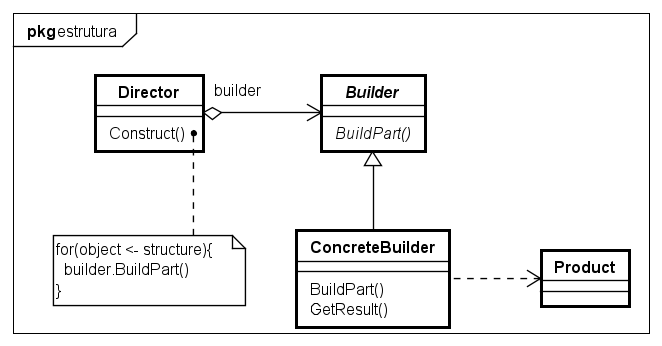
\includegraphics[scale=0.5]{5_padroes-contexto-funcional/5.1_criacionais/5.1.3_builder/builder_estrutura.png}
	\end{center}
\end{figure}

\subsection*{Exemplo Orientado a Objetos}

Como exemplo, podemos observar um leitor de 
documentos do tipo RTF (\textit{Rich Text Format}), 
que deve permitir a conversão de documentos RTF 
para outros formatos, como texto em ASCII ou em um 
\textit{widget} de texto que pode ser editado de 
forma interativa. Como a quantidade de formatos 
possíveis é grande, deve ser possível adicionar 
novos formatos sem que seja necessário modificar 
a classe do leitor de documentos RTF. 

O diagrama de classes apresentado na imagem 
\ref{builder_exemplo} demonstra o uso do padrão 
Builder para esse exemplo. Para cada formato possível 
de conversão, uma nova classe Builder é criada. 
As classes ASCIIConverter, TeXConverter e 
TextWidgetConverter representam, respectivamente, 
os \textit{builders} para os conversores para texto 
em ASCII, LaTeX e \textit{widget} de texto interativo. 
A classe RTFReader chama as operações de construção 
dos conversores desejados. O exemplo de 
implementação dessa abordagem é apresentado no 
código \ref{oobuilder}.

\begin{figure}[htb]
	\caption{\label{builder_exemplo}Exemplo de Builder}
	\begin{center}
	    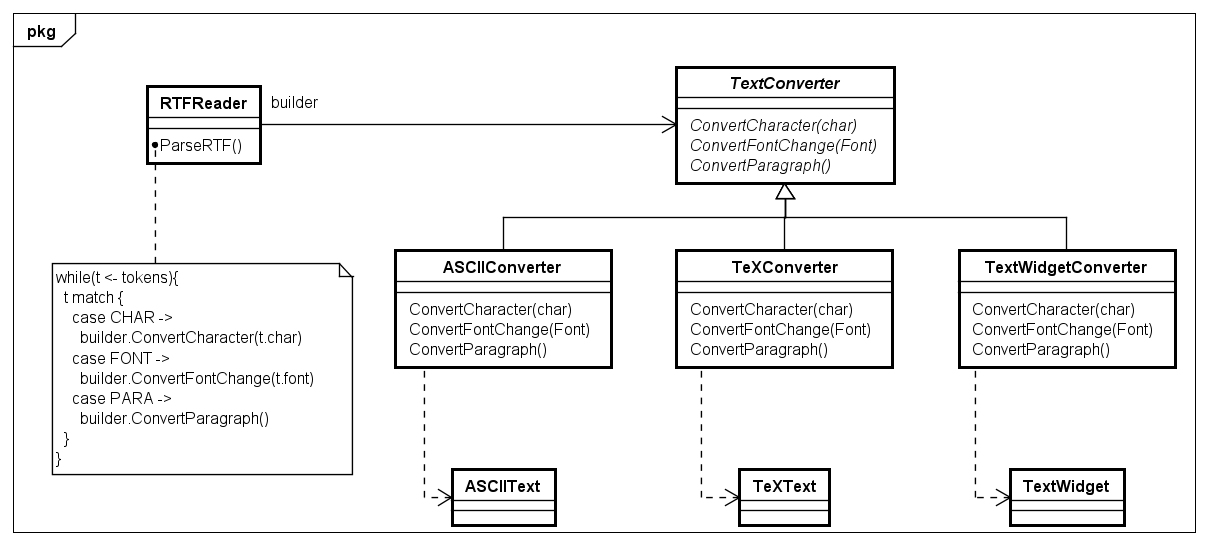
\includegraphics[scale=0.5]{5_padroes-contexto-funcional/5.1_criacionais/5.1.3_builder/builder_exemplo.png}
	\end{center}
\end{figure}

\begin{lstlisting}[caption={Builder Orientado a Objetos},label=oobuilder]

trait TextConverter {
  def ConvertCharacter(char : Char)
  def ConvertFontChange(font : String)
  def ConvertParagraph()
} 

class ASCIIConverter(val asciiText: ASCIIText) extends TextConverter {

  def ConvertCharacter(char : Char): Unit = {
    //Converter char
  }

  def ConvertFontChange(font : String): Unit = {
    //Converter fonte
  }

  def ConvertParagraph(): Unit = {
    //Converte parágrafo
  }
}

class TeXConverter(val texText : TeXText) extends TextConverter {
  def ConvertCharacter(char: Char): Unit = {
    //Converter char
  }

  def ConvertFontChange(font : String): Unit = {
    //Converter fonte
  }

  def ConvertParagraph(): Unit = {
    //Converte parágrafo
  }
}

class TextWidgetConverter(val textWidget: TextWidget) extends TextConverter {
  def ConvertCharacter(char: Char): Unit = {
    //Converter char
  }

  def ConvertFontChange(font : String): Unit = {
    //Converter fonte
  }

  def ConvertParagraph(): Unit = {
    //Converte parágrafo
  }
}

class RTFReader(var textConverter: TextConverter) {

  def SetTextConverter(textConverter: TextConverter): Unit = {
    this.textConverter = textConverter
  }

  def ParseRTF(): Unit = {
    val tokens : List[Token] = List()
    // ...
    for(t <- tokens) {
      t.Type match {
        case TokenType.CHAR => textConverter.ConvertCharacter(t.Character)
        case TokenType.FONT => textConverter.ConvertFontChange(t.Font)
        case TokenType.PARAGRAPH => textConverter.ConvertParagraph()
      }
    }
    // ...
  }
}

\end{lstlisting}

\subsection*{Contexto Funcional}

É possível aproveitar as funções de alta ordem 
da programação funcional para simplificar o 
padrão Builder. Ao invés de definir novas 
classes para cada tipo de builder, uma função 
pode receber como 
parâmetro as operações de construção desejadas. 
No código \ref{fpbuilder}, essa função é a 
ParseRTFBuilder, definida na linha 2. 
Para facilitar o reuso de tipos diferentes 
de \textit{builder}, ela retorna uma nova 
função que recebe como parâmetro uma 
lista de \textit{tokens} e 
retorna uma nova lista no formato desejado. 

A função retornada é análoga ao método 
ParseRTF da classe RTFReader do exemplo 
orientado a objetos. Com essa implementação, 
para cada variação de \textit{builder}, 
basta executar a função 
ParseRTFBuilder passando as operações 
desejadas. Isso pode ser visto na linha 16, 
onde o valor ParseRTFToASCII é o resultado 
da definição do \textit{builder} que converte 
RTF em texto no formato ASCII.

\begin{lstlisting}[caption={Builder Funcional},label=fpbuilder]
    
def ParseRTFBuilder(convertCharacter : Char => Token,
             convertFontChange : String => Token,
             convertParagraph : String => Token)
: List[Token] => List[Token] = (tokens : List[Token]) => {
  val parseRest = (tokens : List[Token]) => ParseRTFBuilder(convertCharacter, convertFontChange, convertParagraph)(tokens)
  // ...
  tokens.head.Type match {
    case TokenType.CHAR => convertCharacter(tokens.head.Character) :: parseRest(tokens.tail)
    case TokenType.FONT => convertFontChange(tokens.head.Font) :: parseRest(tokens.tail)
    case TokenType.PARAGRAPH => convertParagraph(tokens.head.Paragraph) :: parseRest(tokens.tail)
  }
  // ...
}

val ParseRTFToASCII = ParseRTFBuilder(
              ConvertASCIICharacter,
              ConvertASCIIFontChange,
              ConvertASCIIParagraph)
    
\end{lstlisting}